\chapter{Atomistic Simulations of Si Nanoparticles}

In this Appendix we report the technical and methodological aspects of the various atomistic simulations utilized in our studies of Si nanoparticles (NPs).

\section{Density Functional Theory Calculations on Pressurized Si Nanocrystal Structures}
In chapter 5, we utilize DFT calculations to establish that the origin of photoluminescence from Si NPs lies in delocalized band-edge states which shift with pressure in the same manner as the indirect-gap band-edge transition in bulk Si. 

\subsection{Choice of Exchange Correlation Functional}
The Generalized Gradient Approximation (GGA) exchange-correlation (XC) functional from Perdew, Burke, and Ernzerhof (PBE) \cite{PhysRevLett.77.3865} was chosen for most of our DFT calculations to maintain a balance of accuracy and computational efficiency. However, the PBE XC functional suffers from the well-known self-interaction error (SIE), wherein cancellation of the Coulomb self-interaction is incomplete. This tends to result in spurious delocalization of electron density and underestimation of semiconductor bandgaps  \cite{cohen2008insights, PhysRevLett.100.146401}. Because we are interested in examining the shift of Si NP energy gap with pressure and in examining the charge density associated with the band-edge states, we must first ascertain that the PBE functional is appropriate for this system. Here we present a benchmark study of smaller systems utilizing the hybrid XC functional due to Heyd, Scuseria, and Ernzerhof (HSE), which utilizes exact Hartree-Fock exchange for short-range exchange interactions and significantly improves accuracy. This added accuracy comes at increased computational cost, however, with HSE calculations being 50-1000 times more expensive than PBE calculations. For this reason, we utilize a CH$_3$-passivated Si(111) surface as a model system, depicted in Figure \ref{f:sidft1}.

\begin{figure}
\begin{center}
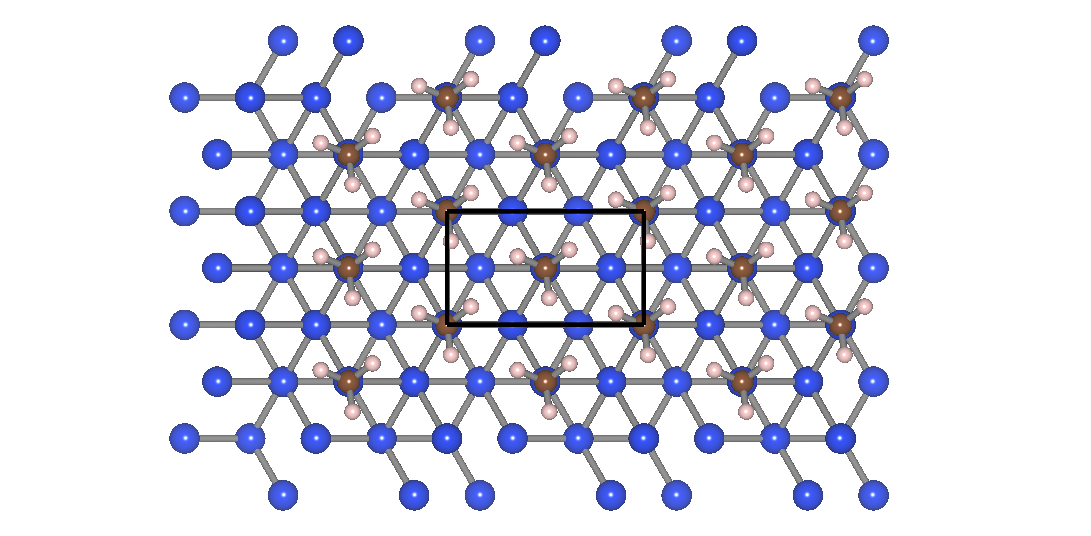
\includegraphics[width=0.75\textwidth]{./appendixD/sidft1.png}
\caption[CH$_3$-passivated Si(111) model system to test XC functional dependence of DFT results.]{CH$_3$-passivated Si(111) model system to test XC functional dependence of DFT results. The simulation cell is shown in the black rectangle.}
\label{f:sidft1}
\end{center}
\end{figure}

\subsubsection{Effect of Strain} To test the impact of lattice strain (conceptually similar to pressurizing the nanocrystal), Si-Si bonds were manually shortened by a constant percentage and CH$_3$ atomic positions were relaxed following each adjustment. For each strain, the HOMO-LUMO gap was calculated using the PBE and HSE XC functionals. Figure \ref{f:sidft2}(a) compares the strain dependence of the HOMO-LUMO gap for each XC functional.

\begin{figure}
\begin{center}
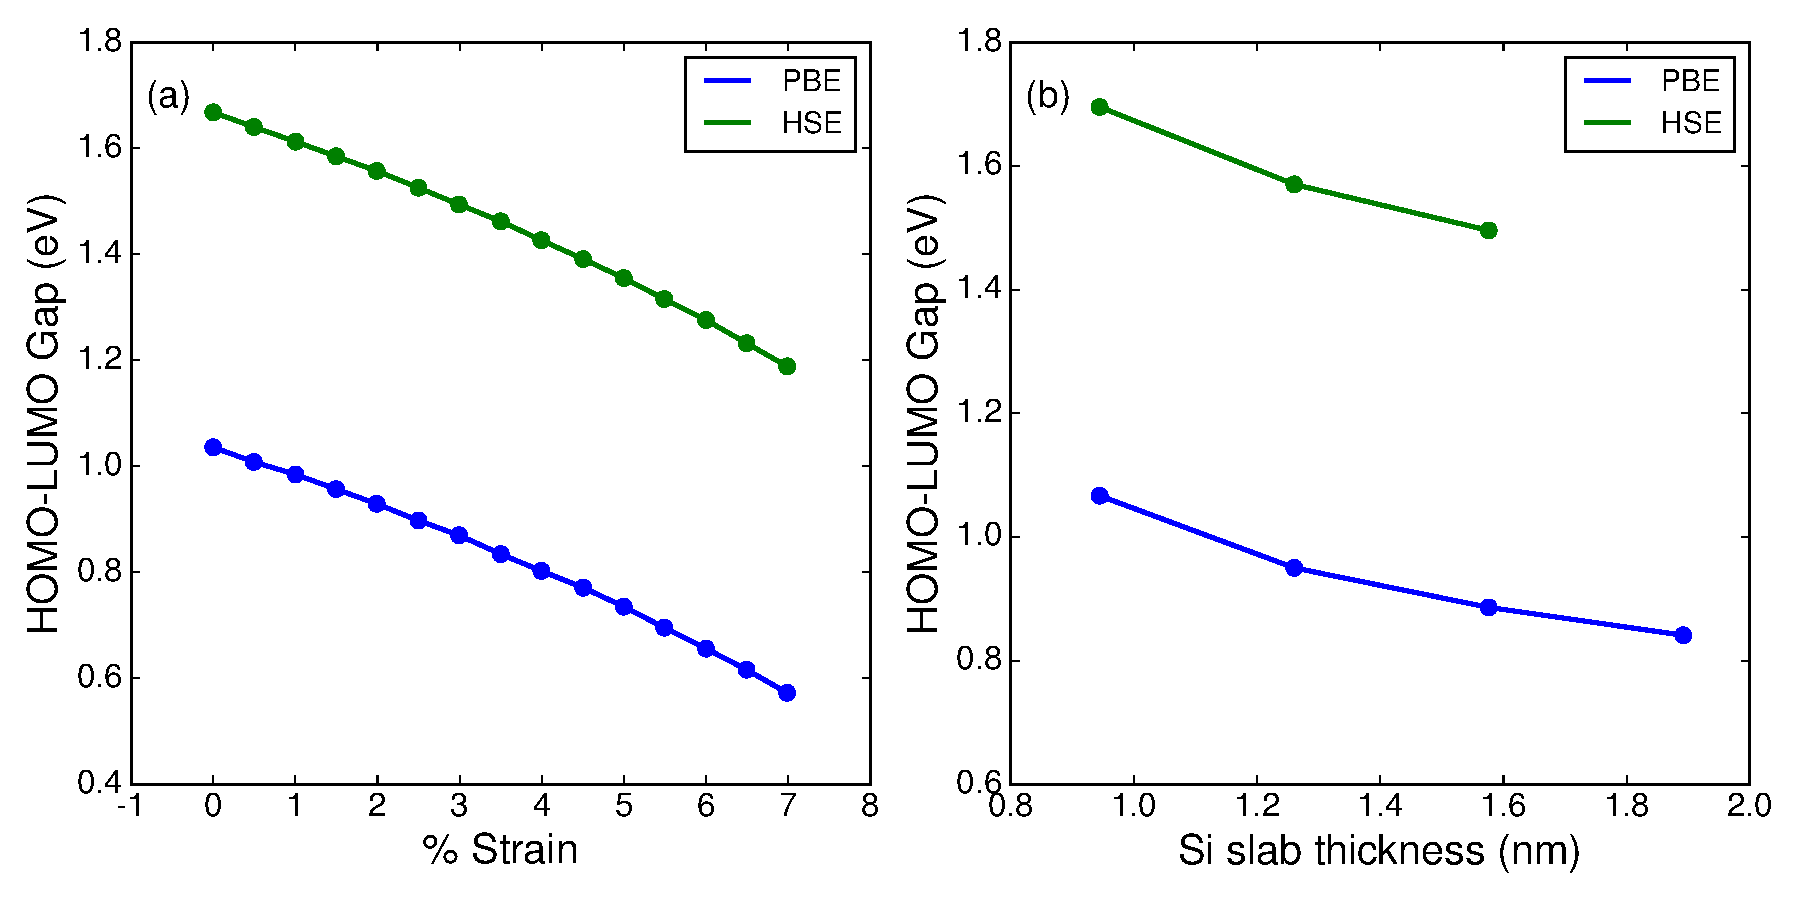
\includegraphics[width=\textwidth]{./appendixD/sidft2.pdf}
\caption[Comparison of XC functionals for modeling strain and size dependence of NC electronic structure.]{(a) The dependence of HOMO-LUMO gap on strain for a 9.5\r{A} thick, CH$_3$-passivated Si(111) slab.  Results for the PBE and HSE functionals are shown. (b) The dependence of HOMO-LUMO gap on Si slab thickness for a CH$_3$-passivated Si(111) slab.}
\label{f:sidft2}
\end{center}
\end{figure}

\subsubsection{Effect of Quantum Confinement} As the study in chapter 5 examines multiple sizes of Si NP, the sensitivity of band edge states to quantum confinement is of interest. We test this effect by computing the HOMO-LUMO gap as a function of Si slab thickness, the results of which are shown in Figure \ref{f:sidft2}(b). As expected, thicker slabs exhibit a small HOMO-LUMO gap, and importantly, the difference between the two functionals is roughly constant.

\subsection{Conclusions} The results presented in Fig. \ref{f:sidft2} suggest that band-edge states respond comparably to strain and quantum confinement between the PBE and HSE XC functionals. This enforces the validity of utilizing the PBE XC functional in our calculations on pressurized Si NPs. While the band gap magnitude is underestimated, trends are likely to be correctly captured. 

\section{Molecular Dynamics Simulations of Hybrid Amorphous/Crystalline Si Nanoparticles}
To further explore the effects of the amorphous shell proposed in chapter 5, we carried out simulations of Si NP lattice dynamics using a Tersoff potential \cite{PhysRevB.37.6991}, which has been shown to reproduce well the structural \cite{chen2012molecular, PhysRevB.37.6991}, thermal \cite{jiang2013modulation} and mechanical \cite{zhang2011deformation} properties of bulk and nanocrystalline silicon. 

\subsection{Structure Generation and Optimization}
A faceted Si NP having a diameter of 4 nm was created via the well-known Wulff construction, using the following surface energies \cite{hong1998effect}: E$_{111}$ = 2.57 eV/m$^2$, E$_{110}$ = 3.72 eV/$m^2$, E$_{100}$ = 3.49 eV/m$^2$. Interatomic forces were first relaxed using the Broyden-Fletcher-Goldfarb-Shanno algorithm \cite{fletcher2013practical}. Following structural optimization, phonon frequencies were calculated from the dynamical matrix, $D$. The corresponding eigenvectors, which give the displacements associated with a particular phonon mode, were also computed. The dynamical matrix is given by Equation \ref{eq:simd1}:
\begin{equation}\label{eq:simd1}
D_{i\alpha j\beta}(k) = \frac{1}{\sqrt{m_im_j}}F_{i\alpha j\beta}(k)
\end{equation}
The force constant matrix, $F$, was calculated according to Equation \ref{eq:simd2}:
\begin{equation}\label{eq:simd2}
F_{i\alpha j\beta}(k) = \sum_{R}\left(\frac{\partial^2U}{\partial\alpha\partial\beta}\right)\exp{\left[ik\left(r_{ij} + R\right)\right]}
\end{equation}
In the above equations, $k$ is phonon wavevector, $U$ is the total internal energy of the Si NP, $m_i$ is the mass of atom $i$, $\alpha$ and $\beta$ vary over all Cartesian atomic coordinates, and $r_{ij}$ is the distance between atoms $i$ and $j$. The phonon frequencies, $\omega$, are the solutions of the secular equation in Equation \ref{eq:simd3}:
\begin{equation}\label{eq:simd3}
|D_{i\alpha j\beta} - \omega^2\delta_{\alpha\beta}\delta_{ij}| = 0
\end{equation}
In Equation 3, the vertical brackets represent the determinant operator. A $70 \times 70 \times 70$ \r{A} simulation box was used; these dimensions are large enough to fully contain the 4 nm-diameter Si NP and prevent the structure from interacting with its periodic images. Calculations were carried out at the $\Gamma$-point in the Brillouin zone. Amorphous Si NPs having the same number of atoms were generated by quenching particles from a molten state. To generate molten Si NPs, crystalline Si NPs, constructed as described above, were first equilibrated at a temperature of 100 K for 12 ps in the NVT ensemble. The temperature was then ramped to 2500 K in steps of 100 K, with 12 ps of equilibration at each temperature step. After annealing to 2500 K, the temperature of the particle was quenched to 300 K and further equilibrated for 12 ps. Finally, amorphous structures were sampled from a 8 ps simulation in the NVE ensemble following the quenching step. Core-shell structures were generated by defining a core radius ($r_{core}$). Particles having a distance $r$ from the particle center less than the core radius ($r < r_{core}$) were held at 300 K for the duration of the temperature ramping, while particles outside the core radius ($r > r_{core}$) were subject to the melt-quench routine described above. The resulting particles possess a crystalline Si core and an amorphous Si shell. Phonon frequencies and eigenvectors for these core-shell particles were computed as described above. All MD simulations in this section were carried out using the General Utility Lattice Program (GULP) \cite{gale2003general}.

\subsection{Vibrational Density of States (VDOS)}
Figure \ref{f:simd1} compares the phonon frequency spectrum (VDOS), obtained as described above, for crystalline Si NPs, amorphous Si NPs, and core-shell structures comprising shell thicknesses corresponding roughly to 2- and 3-monolayer amorphous shells. The VDOS spectrum for crystalline Si NPs exhibits all of the modes found in bulk, crystalline Si. The spectrum shows an intense, sharp peak at $\sim$500 cm$^{-1}$ corresponding to the transverse optical (TO) phonon mode, while broader peaks at $\sim$450 cm$^{-1}$, $\sim$350 cm$^{-1}$, and $\sim$200 cm$^{-1}$ correspond to the longitudinal optical (LO), longitudinal acoustic (LA), and transverse acoustic (TA) phonon modes \cite{dolling1966thermodynamic} These assignments are indicated in Figure S3. The VDOS for an amorphous Si NP is considerably broadened, with no sharp peak corresponding to the TO phonon mode. A 3-monolayer amorphous shell has a VDOS spectrum which is predominantly amorphous, while the 2-monolayer amorphous shell exhibits vestiges of the purely crystalline particle with a broadened TO-like peak at $\sim$500 cm$^{-1}$. 

\begin{figure}
\begin{center}
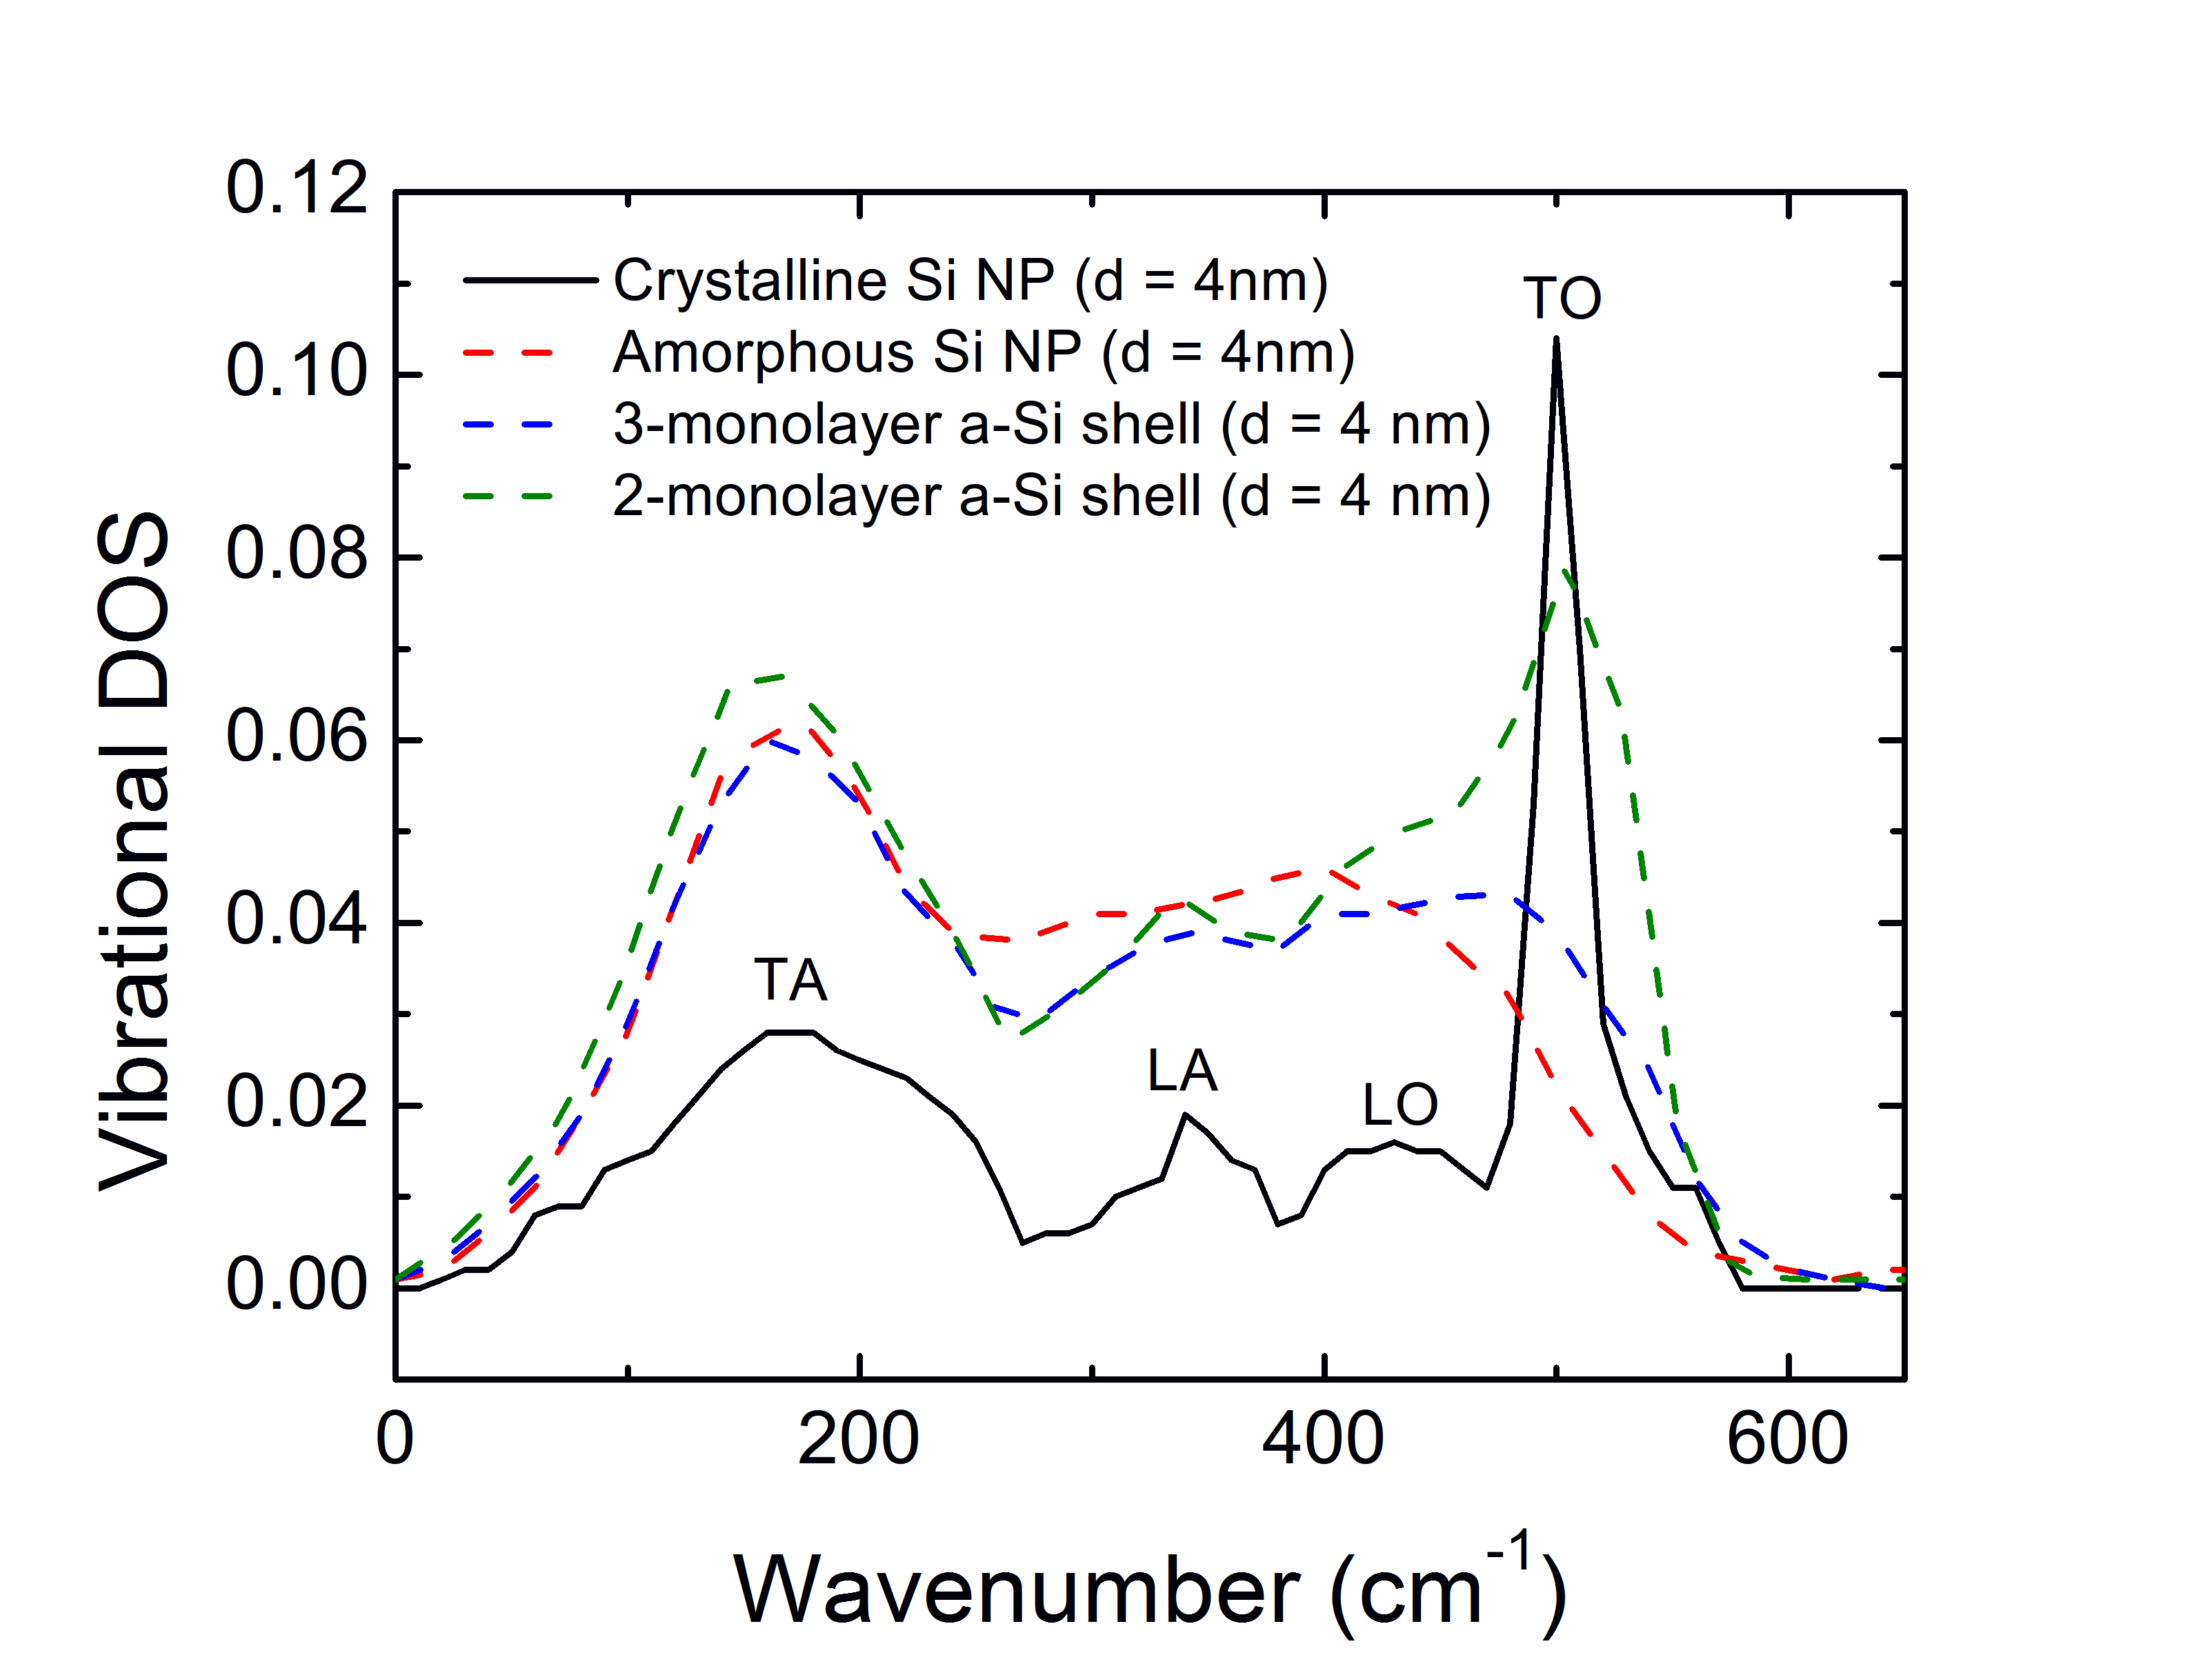
\includegraphics[width=0.75\textwidth]{./appendixD/simd1.png}
\caption[Vibrational density of states for core-shell amorphous-crystalline Si NPs.]{The vibrational density states (VDOS) for Si NPs as obtained from Tersoff-MD-derived dynamical matrices. The fully crystalline Si NP (solid black line) presents modes which clearly correspond to the phonon modes of bulk Si (TO, LO, LA, TA); these are indicated on the figure. As increasing amounts of amorphous material (a-Si) are added, the VDOS broadens markedly, with the TO mode gradually disappearing and the lower frequency modes broadening and gaining intensity.}
\label{f:simd1}
\end{center}
\end{figure}

\subsection{Molecular Dynamics-derived Raman Scattering Spectra}
Using the VDOS and phonon eigenvectors obtained using the procedure described above, we calculated the resonance Raman scattering spectra using the assumption that the Raman intensity in mode $i$ is proportional to $2S_i\omega^2$, where $S_i$ is the Huang-Rhys parameter for mode $i$. Although resonance Raman intensities technically depend on electron-phonon coupling in a complex fashion, the approximation that $I_{Raman}(\omega) \propto 2S_i\omega^2$ has been found to be an effective approximation for low-frequency vibrations and broad electronic spectra \cite{harris1983simple, doi:10.1021/nn201475d}. We further approximate that the Huang-Rhys parameter is the same for each mode in the system and obtain the Raman scattering spectra presented in Figure \ref{f:amsi3} of the manuscript. 
